\section{Durchführung}

In dem Experiment wird der in Abbildung \ref{fig:aufbau} dargestellte Aufbau
verwendet.

\begin{figure}[H]
  \centering
  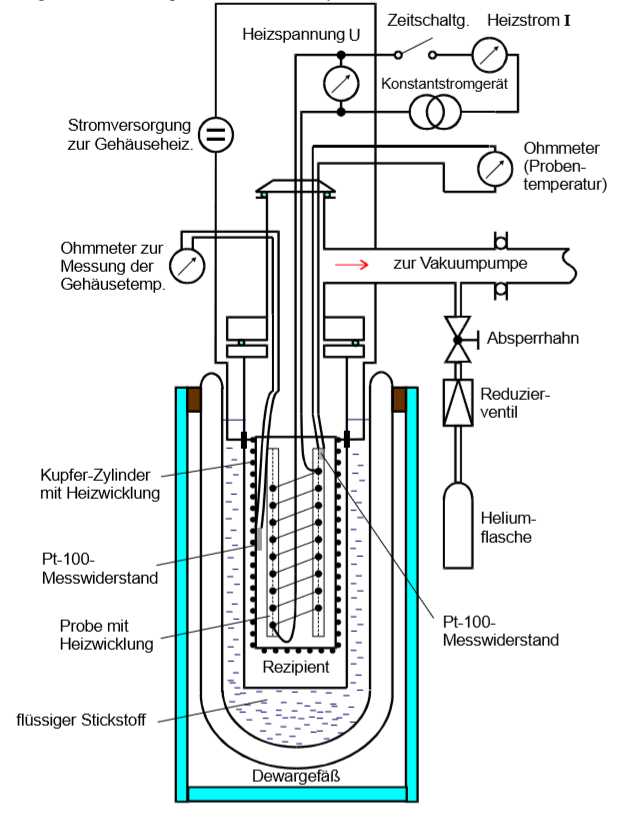
\includegraphics[width=10cm]{aufbau.png}
  \caption{In dem experiment verwendeter Aufbau \cite{skript}}
  \label{fig:aufbau}
\end{figure}

Zu Beginn der Messung wird der Rezipient evakuiert und dann mit Helium gefüllt.
Das Dewar-Gefäß, das den Rezipienten umgibt, wird dann mit flüssigem
Stickstoff gefüllt, damit der Rezipient die Temperatur von dem Stickstoff, also
ungefähr $\SI{80}{\kelvin}$, annimmt. Der Vorgang der Temperaturübertragung
dauert ungefähr $\SI{1}{\hour}$. Danach wird der Rezipient erneut evakuiiert,
um Wärmeverlust durch Konvektion zu vermeiden. Die kalte Probe im Rezipienten
wird dann mit Hilfe einer Heizwicklung erwärmt, ihr wird also elektrische
Energie zugeführt. Zur Messung der Temperatur wird ein Thermoelement verwendet,
welches einen Widerstand misst.

Energieverluste können in diesem Versuch nicht nur durch Konvektion, also
den Wärmeverlust durch Teilchenströme, entstehen. Ein weiterer Energieverlust
ist durch Wärmestrahlung gegeben. Wird die Probe erhitzt, so gibt strahlt sie
Wärme ab. Um diese Verluste zu minimieren, wird um die Probe ein Gehäuse
gestellt, welches auf die Temperatur der Probe geregelt wird. Dadurch strahlt
auch dieses Gehäuse Wärme ab, welches von der Probe wieder aufgeommen wird.
Dadurch sollte bei optimaler Abstimmung der Wärmeverlust durch Wärmestrahlung
verringert werden. Zudem kann Energie durch Wärmeleitung an die Bauteile
verloren gehen.
